\chapter{Plugin továbbfejlesztése}

Ebben a fejezetben ismertetem a beépülő modulon végzett továbbfejlesztéseket melyeket a mesterképzés során végeztem. 

\section{Fejlesztés céljai}

A fejlesztés során hozott alkalmazott megoldások áttekintése előtt érdemes végigvenni, hogy mik is voltak a fejlesztés fő céljai és mi volt ezeknek a motivációja.

\subsection{Funkcionális dekompozíció transzformálása}
Egy rendszert állapotait és állapotváltásait le lehetne modellezni egy mindent tartalmazó állapotgéppel, párhuzamos régiókkal és egyéb modellezési megoldásokkal. Ahogy a modell mérete nő a funkcionalitást érdemes feldarabolni és részenként modellezni. Ez nem csak az áttekinthetőséget segíti, de megkönnyíti a modellen való csapatmunkát is a mérnökök számára hiszen a szétbontott részeket külön, egymástól független lehet modellezni, majd ezeket összekapcsolni.

Szerencsére a Gamma erre a problémára is megoldást kínál, támogatja az állapot dekompozíció modellezését és formális verifikációját.

\subsection{Eredmények megjelenítése}
Fontos kérdés, hogy a formális verifikáció eredményét milyen formában kívánjuk megjeleníteni a mérnökök számára. A plugin eddigi verziója csak arra a kérdésre tudott választ adni, hogy teljesülnek-e a modellel szemben támasztott megkötések vagy sem.

Az \uppaal és a Gamma is képes sokkal részletesebb választ adni. Ezt a Gamma Back-annotation formájában teszi azaz a verifikációban előállt időzítések és lépéseket visszavezeti az eredeti modellbe. Ehhez a Gamma egy elég jól értelmezhető nyelvtant definiál, azonban a SysML-t jellemzően rendszermérnökök használják akik inkább a diagramokat mint a szöveges leírásokat preferálják általában.

A Back-annotationt úgy is lehet interpretálni mint lépések egy sorozatát, amelyek szinkron esetben egymást jól meghatározható sorrendben követik. Ezt leginkább szekvencia diagramokon lehet ábrázolni. Ezen felül ami miatt még a szekvencia diagram tűnik a legkézenfekvőbb megjelenítési megoldásnak az a MagicDraw, illetve a Cameo Simulation toolkit. Ez ugyanis képes szimulációt rögzíteni szekvencia diagramok formájában (\refstruc{fig:md-cameo-rec})) és ezeket újra lejátszani. A cél tehát olyan szekvencia diagramok előállítása úgy minthogyha a szimulátort használva találtuk volna meg a hibautakat, így ezekről nem csak egy jól áttekinthető megoldást kapunk szekvenciák formájában, hanem ezek szimulálhatók is lesznek Cameo Simulation Toolkit segítségével.

\begin{figure}[!ht]
	\centering
	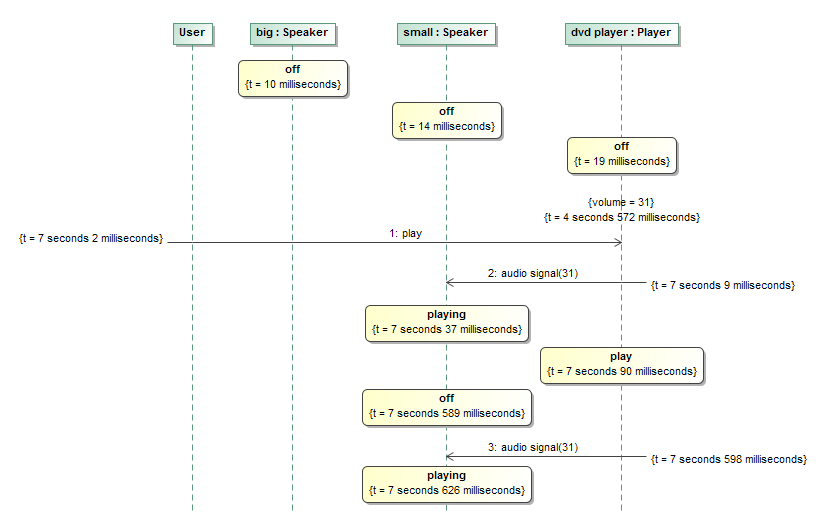
\includegraphics[width=140mm, keepaspectratio]{figures/contribution/md-cameo-rec.png}
	\caption[]{Rögzített szimuláció szekvencia diagramon\footnotemark}
	\label{fig:md-cameo-rec}
\end{figure}

\footnotetext{Forrás: https://docs.nomagic.com/display/CSTD184/Recording+simulation+as+a+Sequence+diagram}

\subsection{Követelmények definiálása}

A formális verifikáció elvégzéséhez a modelleken felül meg kell tudnia a felhasználónak azokat a kérdéseket melyekre választ szeretne kapni a modell ellenőrzése során. Ezek jelen esetben a "Kerülhet-e a rendszer adott állapotba" illetve "Adott állapotból el tud-e jutni egy másikba" típusúak jellemzően. Az \uppaal-ban ezeket temporális logikai kifejezések segítségével tudjuk megtenni \uppaal Queryk formájában ezért ezeket az ellenőrzés során elő kell állítanunk.

Eredetileg szándékoztam erre egy saját nyelvtant is fejleszteni, de a Gammához időközben készült egy úgynevezett \emph{Property Language} és ez ennek az \uppaal-ra transzformáló funkciója és végül ezt használtam fel.

\subsection{Validáció}

A fejlesztés során hozott számos döntés megköveteli, hogy a modellekre vonatkozzanak bizonyos jól-formáltsági kényszerek. Ezek egy része a Gammából örökölt. Például a \emph{Property Language} egy komponensen belül egy állapotra a régión keresztül tudunk hivatkozni (\emph{[component]+.region.state}). Ebből következik, hogy a régióknak a MagicDraw modellben nevet kell adni, illetve, hogy ezek egyediek legyenek egy állapottérképen belül.

A dolgozat célja egy validációs szabálykészlet létrehozása ami segít a felhasználóknak az eszköz helyes használatában.

\newpage

\section{Gamma UML profil}

A dolgozat elkészítéséhez pusztán a SysML nyelv nem volt elegendő ugyanis szükséges volt  a modellben is eltárolni  bizonyos információkat, mint például az ellenőrizendő követelmények, a Back-annotation, vagy éppen, hogy milyen kompozit szemantikát kívánunk érvényesíteni az adott modellekre.

Ezek információk modellezhetőségéhez készítettem egy MagicDraw profilt. Ez alapvetően három részből áll:

\begin{itemize}
	\item Kompozit szemantika
	\item Check modell
	\item Back-annotation modell
\end{itemize}

Az UML profil érdekessége, hogy tartalmazásokat csak megkötés szintjén \emph{Customization}on keresztül tudunk megadni. UML profil diagramon csak öröklést és \emph{tag}eket van lehetőségünk definiálni.



\subsection{Kompozit szemantika}

A Gamma háromféle komponens végrehajtási szemantikát biztosít a felhasználók számára. Ugyan ezt implicit módon is meg lehet határozni, például a kommunikáció típusából, mégis fontos lehet ezek egyértelmű jelölése. Ezért az UML profil (\refstruc{fig:comp-prof}) a SysML nyelvet kiegészíti néhány sztereotípiával melyek segítségével explicit jelölhetők, hogy milyen szemantikát szeretne a felhasználó érteni Blokkjain.

\begin{figure}[!ht]
	\centering
	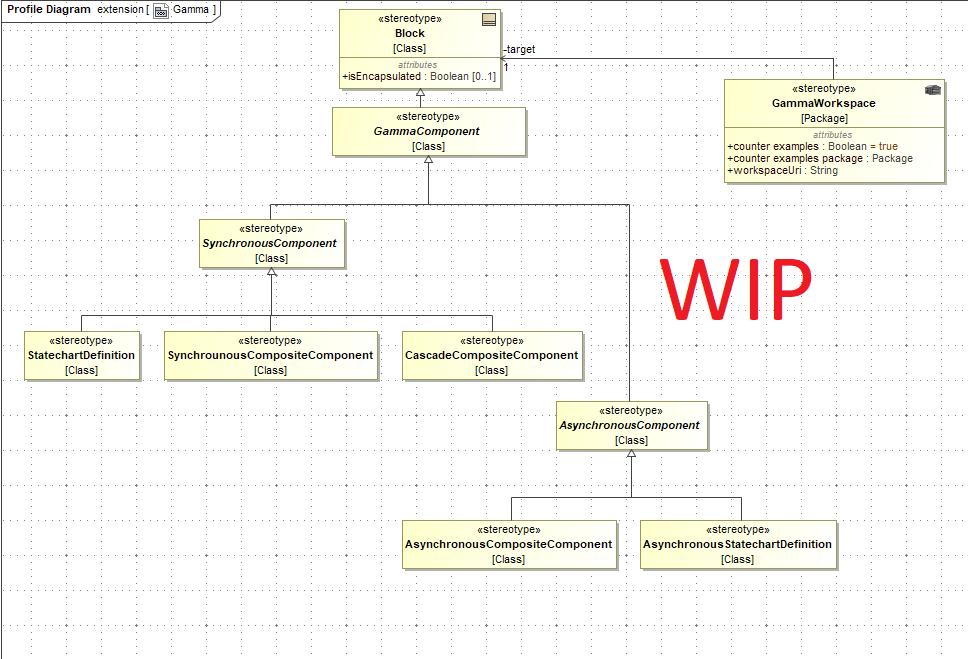
\includegraphics[width=150mm, keepaspectratio]{figures/contribution/profile.png}
	\caption{Szinkron, asszinkron szemantikát támogató UML profil}
	\label{fig:comp-prof}
\end{figure}

A sztereotípiák leszármaznak a Block sztereotípiájából, így lényegében lecserélik azt. Ennek előnye hogy szintaktikailag is asszinkron és szinkron blokkok fognak megjelenni a modelljeinkben. Viszont van egy nagyon nagy hátulütője is mégpedig az, hogyha már meglévő modelleken szeretnénk használni az eszközt ezekhez hozzá kell nyúlni, amihez például elosztott környezetben nem biztos, hogy egyszerű. Ami mégis elfogadhatóvá teszi ezt a plugin jelenlegi iterációjának kapcsán az az őrfeltételek és az akciókra vagy akár az interfészekre vonatkozó megkötések amik - sajnálatos módon - jó eséllyel megkövetelik a modell módosítását.

Egy alternatív megoldás az lehetne, hogy a sztereotípiákat valamilyen él például \emph{Dependency} segítségével rendeljük az egyes komponens definíciókhoz, vagy akár partokhoz. Ez megoldást nyújthat arra a problémára is, hogyha a modell egyes részei külső könyvtárból jönnek, vagy nincs hozzáférésünk hozzájuk.


\subsection{Check modell}

Ahhoz, hogy a formális verifikáció végrehajtható legyen ki kell választani, hogy milyen modelleket szeretnénk ellenőrizni és ezeken milyen követelményeket. Az formális verifikációt modell elemeken keresztül lehet paraméterezni.

Az elképzelés szerint a felhasználó \emph{Workspace}eket hoz létre. Ezek hivatkoznak a felhasználó számítógépén egy könyvtárra melyet az infrastruktúra sajátosságából adódó háttértárra kimentendő modelleket tárolására használok. Ezen felül rajta keresztül kell behivatkozni az ellenőrizendő modellt a projektből.

A modell transzformációk során \emph{Trace}k keletkeznek. Ezek alapján lehet visszakeresni, hogy mely a MagicDraw - Gamma transzformáció során milyen leképzések történtek. Ezek valójában UML propertyk egy \emph{Class}on belül melyeknek a neve egy azonosító amivel a Gamma modell egy kisorosított XMI fájlban lévő elemei vannak hivatkozva. A \emph{property}kből egy \emph{Trace} él mutat a megfelelő MagicDraw elemekre. A kisorosított XMI ugyan ezen \emph{Class} modell elemekhez mint \emph{Comment} vannak hozzárendelve, innen lehet őket kiolvasni.

A követelményeket \emph{GammaProperty} segítségével lehet megadni a Gamma által definiált Property nyelvtan segítségével. Az ezek ellenőrzéséből származó Back-annotaion modellek is a \emph{Workspace}ben helyezkednek el. A modell elemei a következők:
%TODO Update
\begin{itemize}
	\item \textbf{GammaWorkspace} \newline
	Transzformációk és ellenőrzések kezelésére szolgáló MagicDraw projektben tárolt modell.
	\newline
	\textit{Attribútumok:}
	\subitem Target: InstanceSpecification[1]: transzformálandó modell
	\subitem WorkspaceUri: String: egy elérési út a felhasználó egy könyvárához
	\subitem Counter examples: Boolean: Back-annotation engedélyezése
	
	\item \textbf{GammaCheck} \newline
	\emph{GammaProperty}k konténere
	
	\item \textbf{GammaProperty} \newline
	Egy a modellel szemben támasztott követelmény a saját nyelven
	\newline
	\textit{Attribútumok:}
	\subitem body: String[1]: saját nyelven írt kifejezés

	\item \textbf{GammaWorkspaceFile} \newline
	Hivatkozás egy Gamma modellre a háttértáron. A modell elem neve a fájl elérési útja.
	
	\item \textbf{MD2G\_Trace} \newline
	Egy megfeleltetés a MagicDraw és Gamma modellek között. A MagicDraw elemre egy Trace él mutat, a Gammabeli modell elem pedig EMF hivatkozás formájában kerül tárolásra.
	\newline
	\textit{Attribútumok:}
	\subitem URIFragment: String[1]: hivatkozás EMF-es modell elemekre
	
	
\end{itemize}

\subsection{Back-annotation modell}
A back-annotation modell feladata visszacsatolni az eredeti modellbe a valamilyen külső, jellemzően szimulátorból származó időzítési adatokat. A Gamma is készít egy ilyen modellt. A megoldás amit kidolgoztam Gamma modell egy MagicDraw specifikus változatának létrehozásából és egy Gamma-MagicDraw transzformáció megtervezéséből és megvalósításából állt. Az UML profil egy szakterület specifikus nyelvet definiál. Elemei pedig a következők:

\begin{itemize}
	\item \textbf{ExecutionTrace} \newline
	Egy kompozit komponens végrehajtása. \textit{Steppeket} azaz lépéseket tartalmaz, illetve a végrehajtás végén állhat egy lépésekből álló ciklus.
	\newline
	\textit{Attribútumok:}
	\subitem component: InstanceSpecification[1]: kompozit komponens példánya a modellben
	\subitem steps: Step[1..*]: lépések
	\subitem cycle: Cycle[0..1]: lépésekből álló ciklus amire a végrehajtás futhat
	
	\item \textbf{Step} \newline
	A végrehajtás egy lépése. Két részből áll egy \textit{Act} részből, ami a végrehajtódott műveleteket írja le és egy \textit{Assert} részből, ami a lépésben elért állapotot írja le.
	\newline
	\textit{Attribútumok:}
	\subitem actGroup: ActGroup[0..1]: műveletek konténere
	\subitem assert: Assert[1]: lépés során beálló állapotok
	
	\item \textbf{ActGroup} \newline
	\textit{Actok} konténere a \textit{Steppen} belül. Csak áttekinthetőségre szolgál.
	\newline
	\textit{Attribútumok:}
	\subitem acts: Act[0..*]: műveletek konténere
	
	\item \textbf{Act} \newline
	Absztrakt sztereotípia. Egy végrehajtott művelet.
	
	\item \textbf{ComponentSchedule} \newline
	Komponensen egy kör végrehajtása (üzenetek kiolvasása az üzenetsorokból, állapotok léptetése)
	
	\item \textbf{TimeElapse} \newline
	Végrehajtás várakoztatása bizonyos ideig.
	\newline
	\textit{Attribútumok:}
	\subitem value: Integer: várakozás ideje milliszekundumban
	
	\item \textbf{RaiseEventAct} \newline
	Egy esemény elküldése a komponens példánynak.
	\newline
	\textit{Attribútumok:}
	%TODO ez itt biztosan válozik majd
	\subitem referencedAction: Behavior: eseményt küldő viselkedés.
	
	\item \textbf{InstanceState} \newline
	Absztrakt. Az egyes példányok, partok állapotainak leírása.
	\newline
	\textit{Attribútumok:}
	\subitem referencedPart: PartProperty: hivatkozott komponens példány
	
	\item \textbf{InstanceVariableState} \newline
	Egy változónak egy állapota.
	\newline
	\textit{Attribútumok:}
	\subitem referencedVariable: Property: hivatkozott változó
	\subitem value: ValueSpecification: hivatkozott változó értéke
	
	\item \textbf{InstanceStateConstant} \newline
	Az állapot gép egy állapota.
	\newline
	\textit{Attribútumok:}
	\subitem referencedState: State: hivatkozott állapot konstans
\end{itemize}

A \refstruc{fig:contribution-trace-profile} az UML profilt, a \refstruc{fig:contribution-trace-customization} pedig ennek a customizationjét mutatja.

\begin{figure}[!ht]
	\centering
	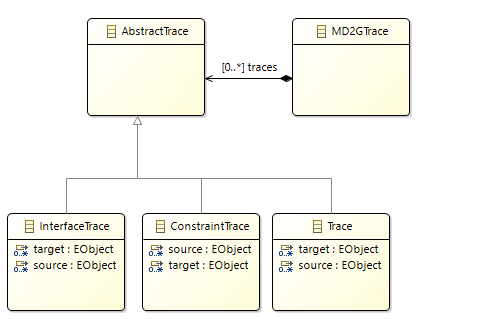
\includegraphics[width=90mm, keepaspectratio]{figures/contribution/trace-model.png}
	\caption{Back-annotation UML profilja}
	\label{fig:contribution-trace-profile}
\end{figure}

\begin{figure}[!ht]
	\centering
	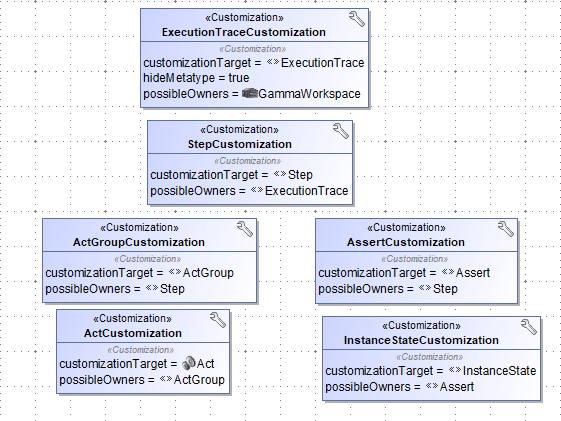
\includegraphics[width=90mm, keepaspectratio]{figures/contribution/trace-profile.png}
	\caption{Back-annotation customization modellje}
	\label{fig:contribution-trace-customization}
\end{figure}
 
 \newpage


\section{Kompozíciók transzformációja}

Egy nagy komplex rendszert célszerű nem egyben, hanem részekre bontva modellezni majd a részek egymáshoz illesztéséből, komponálásából képezni a teljes rendszert. Állapottérképek dekomponálását azaz részekre bontását a Gamma is támogatja. A kihívás a SysML és a Gamma közötti megfeleltetések megválasztása oly módon, hogy a szemantika ne sérüljön. A megfeleltetés két szempontól kell vizsgálni, egyszer az elemek tartalmazási hierarchiái szerint, egyszer pedig a köztük modellezett kommunikáció szerint.



\subsection{Struktúra megfeleltetése}
A Gammában nyelvi szinten elkülönül az állapottérkép (StatechartDefinition) és a kompozit komponens (Composite Component) fogalma. Állapottérképek a modell hierarchia gráfjában a levelekben helyezkednek el. SysML esetében a minden Blokknak lehet viselkedése, jelen esetben állapottérképe. A megfeleltetés elvégzéséhez megkötést fogalmaztam meg mely kétféle blokkot enged meg. A viselkedéssel rendelkező blokkokat és azokat amelyek nem tartalmazhatnak viselkedést csak Part Propertyket. Tehát állapottérképek ebben a modellben is csak levelekben lehetnek.

\begin{figure}[!ht]
	\centering
	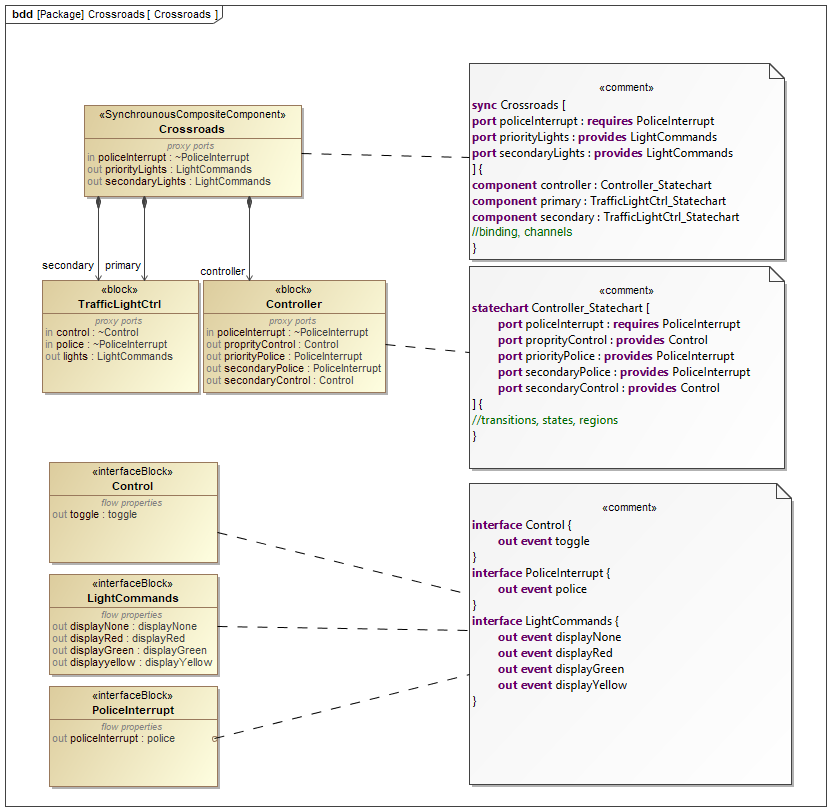
\includegraphics[width=140mm, keepaspectratio]{figures/contribution/md2g.png}
	\caption{Struktúra megfeleltetése}
	\label{fig:md2g}
\end{figure}

Az érdekes kérdés lehet, hogy ha egy magasabb szintű blokknak mégis lehetne viselkedése, azt szemantikailag hogyan kezelhetnénk. Elképzelhető olyan értelmezés, hogy ez a magas szintű állapottérkép a dekomponált részek együttes viselkedését írja le. Ez lehetőséget adna arra, hogy a magasabb és az alacsonyabb szintű viselkedés halmazt összehasonlítsuk működés szempontjából és ha nincsenek szinkronban akkor tervezési hibaként értelmezzük. Így a magasabb hierarchia szintek tulajdonképpen validálnák az alacsonyabb szinteket. Ennek a lehetőségnek a komolyabb kifejtése azonban nem célja a dolgozatnak.

\subsection{Kommunikáció megfeleltetése}

A Gammában a komponensek kommunikációja kimondottan az eseményvezérelt állapot alapú rendszerek sajátosságain alapul, azonban SysML-ben a kommunikáció leírása sokkal általánosabb és többféle módon is modellezhető. Éppen ezért a feladat elvégzése során az események és az interfészek modellezésére megkötéseket kellett megfogalmazni.
Az egyik ilyen megkötés szerint a portokban interfész blokkokat kell tipizálniuk és szinkron szemantika esetében operációkat definiálni, asszinkron esetben pedig szignálokkal tipizált \emph{Flow Property} formájában fel kell tüntetni milyen szignálok fogadására képes a blokk.

Az eseményeknek mindig specifikálniuk kell, hogy melyik porton várják az operáció hívását vagy szignál érkezését. Ez igaz az akciókra az ő esetükben azt kell specifikálni, hogy milyen porton keresztül történjen a küldés.

Portok közül csak a \emph{Proxy} portok támogatottak. Proxy portok iránya származtatott a \emph{Flow property} irányokból amik keresztül mehetnek rajta. Az irány az \emph{isConjugated} flag igazra állításával változtatható.

\section{CTL nyelvtan}

\section{Back-annotation transzformációja}

A Back-annotation egy általában szimulátor által biztosított időzítési adatok visszacsatolása az eredeti modellbe. Ahhoz, hogy MagicDrawban is el tudjuk tárolni ezeket az adatokat létre kellett hoznom egy UML profilt ami a Back-annotation modell metamodelljeként fog szolgálni.

A transzformáció iránya itt megfordul nem MagicDraw modellekből állítok elő Gamma modelleket hanem épp fordítva Gamma modelleket transzformálok MagicDraw modellekké.



\section{Szimuláció}

\section{Példa} %TODO TBD